\section{Auswertung}
\label{sec:Auswertung}
\subsection{Bestimmung des Materials der Stäbe}
\label{sec:Material}
Mit den aus \ref{sec:Stäbe} bekannten Abmessungen ergeben sich die Dichten $\rho$ der Stäbe mittels
\begin{equation}
  \rho = \frac{m}{V} = \frac{m}{Al}
\end{equation}
und
\begin{equation}
  A_r = \pi r^2
\end{equation}
bzw
\begin{equation}
  A_q = a^2
\end{equation}
zu $\rho_r =8397 \frac{kg}{m^3}$  bzw $\rho_q = 8373 \frac{kg}{m^3}$. Es wird somit von Messingstäben ausgegangen.
\subsection{Einseitige Einspannung}
\label{sec:Einseitig}

\begin{table}
  \centering
  \caption{Auslenkung des runden Stabes bei einseitiger Einspannung}
  \label{tab:einseitig-r}
  \sisetup{round-mode = places , round-precision = 3}
  \begin{tabular}{S S S S}
    \toprule
    {$x/cm$} & {$D_o/mm$} & {$D_m /mm$} & {$\Delta D /mm$}\\
    \midrule
  \end{tabular}
\end{table}

\begin{table}
  \centering
  \caption{Auslenkung des eckigen Stabes bei einseitiger Einspannung}
  \label{tab:einseitig-q}
  \sisetup{round-mode = places , round-precision = 3}
  \begin{tabular}{S S S S}
    \toprule
    {$x/cm$} & {$D_o/mm$} & {$D_m /mm$} & {$\Delta D /mm$}\\
    \midrule
  \end{tabular}
\end{table}
\FloatBarrier

Für den runden Stab wurde eine Belastungsmasse von $m_1 = 238.9g$ gewählt, für den eckigen $m_2 = 767.5g$. Ihre Auslenkungen sind in den Tabellen \ref{tab:einseitig-r} und \ref{tab: einseitig-q} aufgelistet. Hierbei bezeichnet $x$ die Position auf dem Stab (Einspannung bei $x = 0$). $D_0$ die Auslenkung im unbelasteten Zustand, $ D_m$ die Auslenkung im belasteten Zustand und $\Delta D$ ihre Differenzen, also die Auslenkung durch die Belastung. Graphisch dargestellt sind die Werte in Abb.\ref{fig:Reihe1} bzw. Abb.\ref{fig:Reihe2}.

\begin{figure}
  \centering
  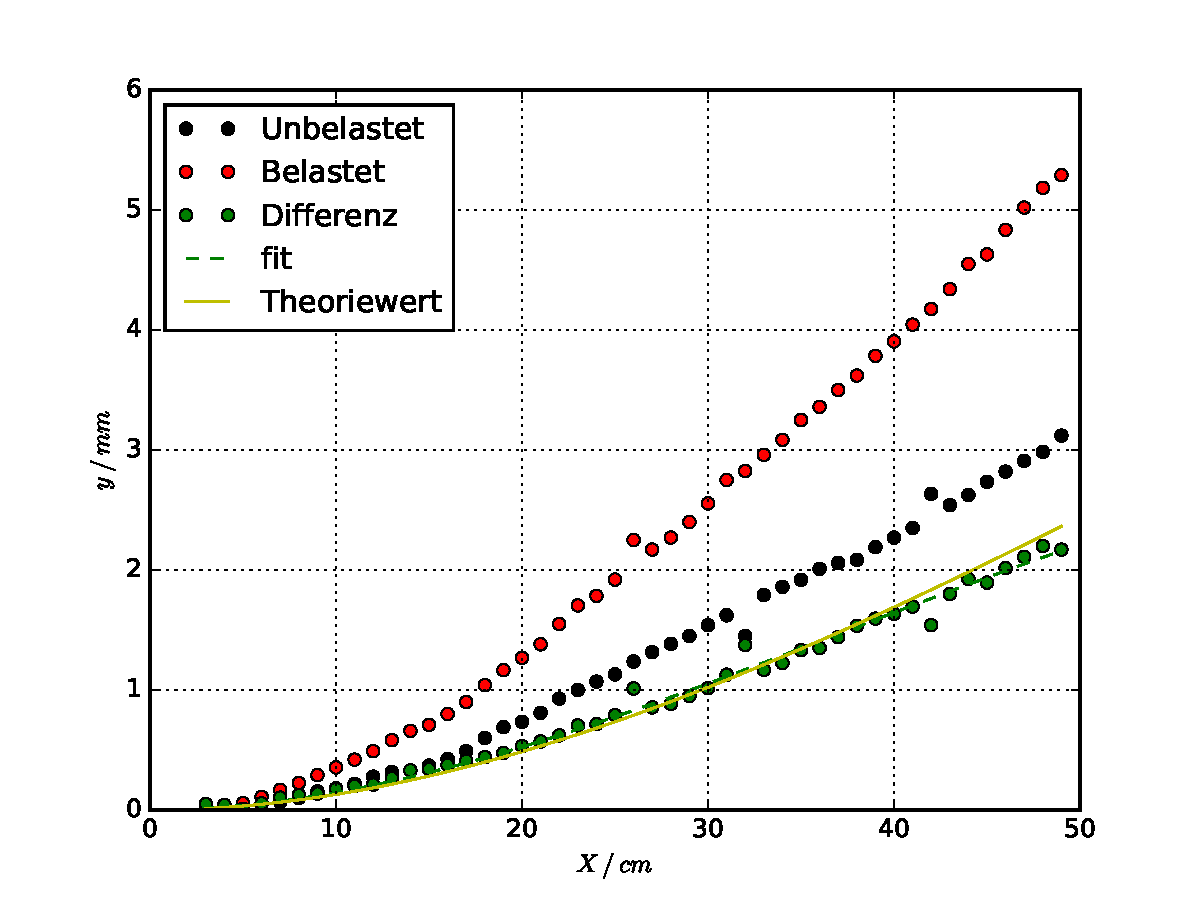
\includegraphics[width = \textwidth]{./Plots/Reihe1.pdf}
  \caption{Auslenkung des runden Stabes, verglichen mit dem Theoriewert}
  \label{fig:Reihe1}
\end{figure}

\begin{figure}
  \centering
  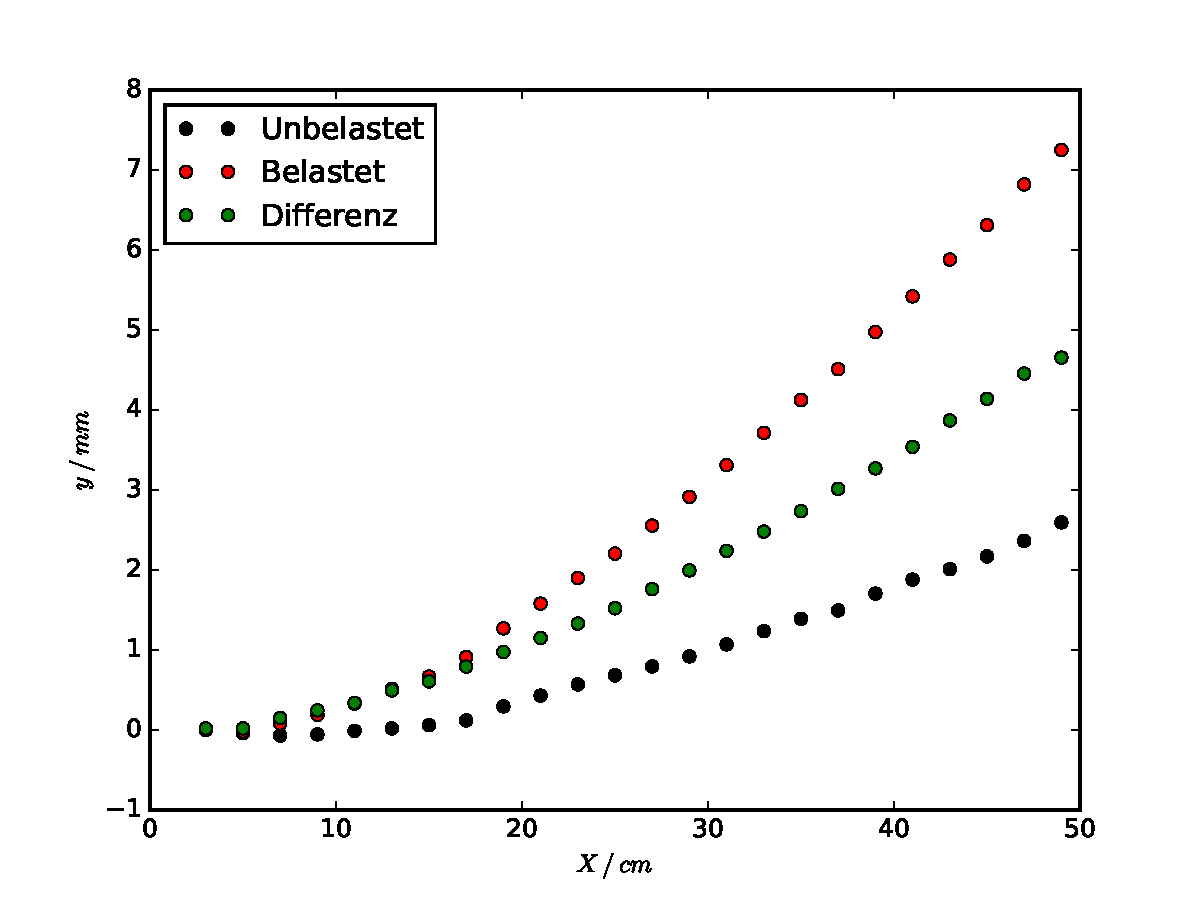
\includegraphics[width = \textwidth]{./Plots/Reihe2.pdf}
  \caption{Auslenkung des runden Stabes, verglichen mit dem Theoriewert}
  \label{fig:Reihe2}
\end{figure}

Die Flächenträgheitsmomente der Stäbe ergeben sich über \eqref{eqn:I} zu
\begin{equation}
  I_r = \frac{\pi}{64}d^4 = 4.9e-10 m^4
\end{equation}
bzw.
\begin{equation}
  I_q = \frac{a^4}{12} = 8.3e-10 m^4
\end{equation}

Mittels dieser Flächenträgheitsmomente und der Auslenkung der Stäbe lässt sich durch \eqref{eqn:D1} das Elastizitätsmodul bestimmen (Tabellen \ref{tab:Er} und \ref{tab:Eq}). Hierraus ergeben sich im Mittel

\begin{equation*}
  E_r = \left(9.76e10 \pm 4.3e9 \right) \frac{N}{m^2}
\end{equation*}
und
\begin{equation*}
  E_q = \left(1.35e10 \pm 6.1 e0 \right) \frac{N}{m^2}.
\end{equation*}

\begin{table}
  \centering
  \caption{$E_r$ berechnet aus $x$}
  \label{tab:Er}
  \sisetup{round-mode = places , round-precision = 2}
  \begin{tabular}{S S}
    \toprule
    {$x/cm$} & {$E_r$}\\
    \midrule
  \end{tabular}
\end{table}

\begin{table}
  \centering
  \caption{$E_q$ berechnet aus $x$}
  \label{tab:Eq}
  \sisetup{round-mode = places , round-precision = 2}
  \begin{tabular}{S S}
    \toprule
    {$x/cm$} & {$E_q$}\\
    \midrule
  \end{tabular}
\end{table}

\subsection{Beidseitige Einspannung}
\label{sec:Beidseitig}
In diesem Versuchsteil ist die Belastung $m_3 = 4722.5g$.
